\documentclass[12pt, a4paper]{report}

% Packages :

\usepackage[french]{babel}
\usepackage[utf8]{inputenc}
\usepackage[T1]{fontenc}
\usepackage[pdftex, pdfauthor={Bacomathiques}]{hyperref}
\usepackage{sectsty}
\usepackage[explicit]{titlesec}
\usepackage{xcolor}
\usepackage{amsmath}
\usepackage{amssymb}
\usepackage{amsthm}
\usepackage{fourier}
\usepackage{titlesec}
\usepackage{fancyhdr}
\usepackage{catchfilebetweentags}
\usepackage[french, capitalise, noabbrev]{cleveref}
\usepackage[fit, breakall]{truncate}
\usepackage[margin=3cm]{geometry}
\usepackage{tocloft}
\usepackage{tikz}
\usepackage{tocloft}
\usepackage{microtype}
\usepackage{listings}
\usepackage{tabularx}
\usepackage{calc}
\usepackage[export]{adjustbox}
\usepackage[most]{tcolorbox}
\usepackage{standalone}
\usepackage{xlop}
\usepackage{etoolbox}
\usepackage{environ}

\usetikzlibrary{arrows.meta}
\usetikzlibrary{trees}

% Paramètres :

\author{Bacomathiques}
\definecolor{graphe}{HTML}{93c9ff}
\setcounter{MaxMatrixCols}{12}
\setlength{\parindent}{0pt}
\setlength{\fboxsep}{0pt}
%\pdfsuppresswarningpagegroup=1

% Code :

\lstdefinestyle{style}{
	backgroundcolor=\color{white},
	commentstyle=\em\color[HTML]{999988},
	keywordstyle=\bfseries,
	identifierstyle=\normalfont,
	stringstyle=\color[rgb]{0.87, 0.07, 0.27},
	basicstyle=\ttfamily\color{black},
	breakatwhitespace=false,
	breaklines=true,
	captionpos=b,
	keepspaces=true,
	numbers=left,
	numbersep=5pt,
	showspaces=false,
	showstringspaces=false,
	showtabs=false,
	tabsize=2,
	numbers=none
}

\lstset{style=style}
\lstset{
	literate=
	{á}{{\'a}}1
	{à}{{\`a}}1
	{ã}{{\~a}}1
	{é}{{\'e}}1
	{ê}{{\^e}}1
	{í}{{\'i}}1
	{ó}{{\'o}}1
	{õ}{{\~o}}1
	{ú}{{\'u}}1
	{ü}{{\"u}}1
	{ç}{{\c{c}}}1
}

\lstset{
	framextopmargin=10pt,
	framexrightmargin=10pt,
	framexbottommargin=10pt,
	framexleftmargin=10pt,
	xleftmargin=10pt,
	xrightmargin=10pt,
}

% Couleurs :

\definecolor{title}{HTML}{912c21}
\definecolor{section}{HTML}{1c567d}
\definecolor{subsection}{HTML}{2980b9}

\definecolor{rule}{HTML}{c4c4c4}

\definecolor{formula}{HTML}{ebf3fb}
\definecolor{formula-left}{HTML}{3583d6}

\definecolor{tip}{HTML}{dcf3d8}
\definecolor{tip-left}{HTML}{26a65b}

\definecolor{demonstration}{HTML}{fff8de}
\definecolor{demonstration-left}{HTML}{f1c40f}

\definecolor{exercise}{HTML}{e0f2f1}
\definecolor{exercise-left}{HTML}{009688}

\definecolor{correction}{HTML}{e0f7fa}
\definecolor{correction-left}{HTML}{00bcd4}

\definecolor{toc}{HTML}{fceae9}
\definecolor{toc-left}{HTML}{e74c3c}
\definecolor{toc-dark}{HTML}{87281f}

% Titres :

\renewcommand{\thesection}{\Roman{section} - }
\renewcommand{\thesubsection}{\arabic{subsection}. }

\newcommand{\sectionstyle}{\normalfont\LARGE\bfseries\color{section}}
\titleformat{\section}{\sectionstyle}{\thesection #1}{0pt}{}
\titleformat{name=\section, numberless}{\sectionstyle}{#1}{0pt}{}

\newcommand{\subsectionstyle}{\normalfont\Large\bfseries\color{subsection}}
\titleformat{\subsection}{\subsectionstyle}{\thesubsection #1}{0pt}{}
\titleformat{name=\subsection, numberless}{\subsectionstyle}{#1}{0pt}{}

\titlelabel{\thetitle\ }

% Table des matières :

\addto\captionsfrench{\renewcommand\contentsname{}}
\renewcommand{\cftsecpagefont}{\color{toc-dark}}
\renewcommand{\cftsubsecpagefont}{\color{toc-dark}}
\renewcommand{\cftsecleader}{\cftdotfill{\cftdotsep}}
\renewcommand{\cftsecfont}{\bfseries}
\renewcommand{\cftsecpagefont}{\bfseries\color{toc-dark}}
\setlength{\cftbeforetoctitleskip}{0pt}
\setlength{\cftaftertoctitleskip}{0pt}
\setlength{\cftsecindent}{0pt}
\setlength{\cftsubsecindent}{20pt}
\setlength{\cftsubsecnumwidth}{20pt}

% Commandes :

\newcommand{\newpar}{\\[\medskipamount]}
\newcommand{\lesson}[3]{%
	\newcommand{\level}{#1}%
	\newcommand{\id}{#2}%
	\hypersetup{pdftitle={#3}}
	\begin{center}%
		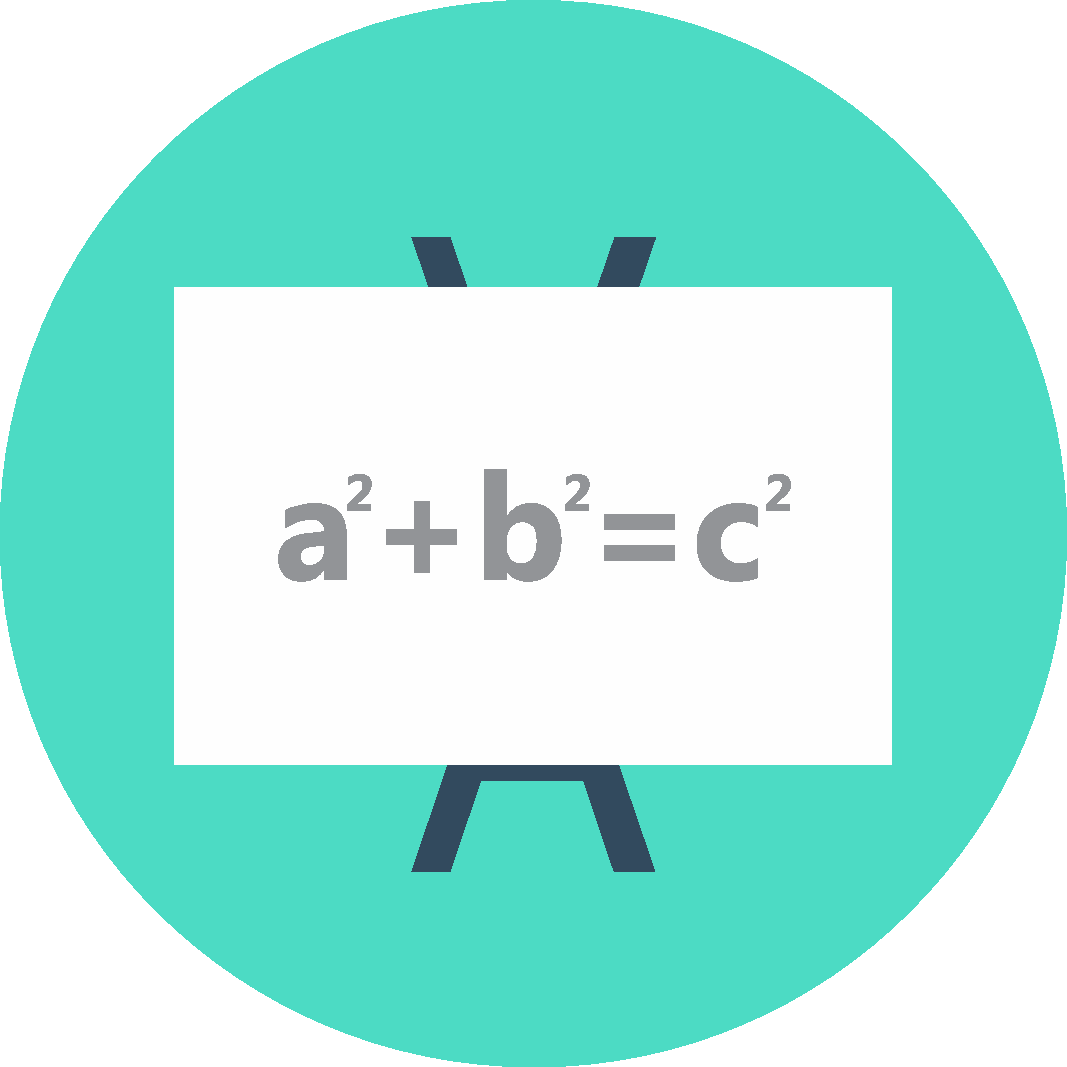
\includegraphics[width=150px]{\imagespath/bacomathiques}%
		
		\vspace{30pt}%
		{\Huge\color{title} #3}%
		
		\vspace{10pt}%
		{Bacomathiques --- \href{https://bacomathiqu.es/cours/#1/#2}{\color{section} https://bacomathiqu.es}}%
		
		\vspace{20pt}%
	\end{center}%
	\begin{toc}
		\tableofcontents%
	\end{toc}
	\thispagestyle{empty}%
	\newpage%
	\setcounter{page}{1}%
}
\newcommand{\imagespath}{../../images}
\newcommand{\lessonimagespath}{\imagespath/lessons/\level/\id/}
\newcommand{\includelatexpicture}[2][\textwidth - 100pt]{%
	\begin{center}%
		\resizebox{#1}{!}{%
			\input{\lessonimagespath#2}%
		}%
	\end{center}%
	\medskip%
}
\newcommand{\includeimage}[1]{%
	\begin{center}%
		\includegraphics{\lessonimagespath#1}%
	\end{center}%
	\medskip%
}
\newcommand{\includerepresentation}[1]{%
	\begin{center}%
		\setlength{\fboxrule}{0.5pt}%
		\href{https://www.geogebra.org/m/#1}{\includegraphics[width=\textwidth-1pt,fbox]{\lessonimagespath#1}}%
	\end{center}%
}
\newcommand{\floor}[1]{\lfloor #1 \rfloor}

\makeatletter
\newcommand\inputcontent{\@ifstar{\inputcontent@star}{\inputcontent@nostar}}
\newcommand{\inputcontent@star}[1]{%
	\ExecuteMetaData[#1]{content}%
}
\newcommand{\inputcontent@nostar}[1]{%
	\newpage%
	\inputcontent@star{#1}%
}
\makeatother

\let\oldsection\section
\renewcommand\section{\clearpage\oldsection}
\newcommand{\contentwidth}[1][medium]{}

% En-têtes :

\pagestyle{fancy}

\renewcommand{\sectionmark}[1]{\markboth{\thesection \ #1}{}}

\fancyhead[R]{\truncate{0.23\textwidth}{\color{title}\thepage}}
\fancyhead[L]{\truncate{0.73\textwidth}{\color{title}\leftmark}}
\fancyfoot[C]{\scriptsize \href{https://bacomathiqu.es/cours/\level/\id}{\texttt{bacomathiqu.es}}}

\makeatletter
\patchcmd{\f@nch@head}{\rlap}{\color{rule}\rlap}{}{}
\patchcmd{\headrule}{\hrule}{\color{rule}\hrule}{}{}
\makeatother

% Environnements :

\newenvironment{nosummary}{}{}
\newcommand{\tcolorboxtitle}[2]{\setlength{\fboxsep}{2.5pt}\hspace{-10pt}\colorbox{#1-left}{\hspace{8pt}\MakeUppercase{#2} \hspace{2pt} \includegraphics[height=0.8em]{\imagespath/bubbles/#1}\hspace{5pt}}}
\newcommand{\tcolorboxsubtitle}[2]{\ifstrempty{#2}{}{\textcolor{#1-left}{\large#2}\\[\medskipamount]}}
\tcbset{
	frame hidden,
	boxrule=0pt,
	boxsep=0pt,
	enlarge bottom by=8.5pt,
	enhanced jigsaw,
	boxed title style={sharp corners,boxrule=0pt,coltitle={white},titlerule=0pt},
	fonttitle=\fontsize{6pt}{6pt}\bfseries\boldmath,
	top=10pt,
	right=10pt,
	bottom=10pt,
	left=10pt,
	arc=0pt,
	outer arc=0pt,
}
\newtcolorbox{toc}[1][]{
	colback=toc,
	borderline west={3pt}{0pt}{toc-left},
	title=\tcolorboxtitle{toc}{Table des matières},
	colbacktitle=toc,
	before upper={\tcolorboxsubtitle{toc}{#1}}
}
\newtcolorbox{formula}[1][]{
	colback=formula,
	borderline west={3pt}{0pt}{formula-left},
	title=\tcolorboxtitle{formula}{À retenir},
	colbacktitle=formula,
	before upper={\tcolorboxsubtitle{formula}{#1}}
}
\newtcolorbox{tip}[1][]{
	colback=tip,
	borderline west={3pt}{0pt}{tip-left},
	title=\tcolorboxtitle{tip}{À lire},
	colbacktitle=tip,
	before upper={\tcolorboxsubtitle{tip}{#1}}
}
\newtcolorbox{demonstration}[1][]{
	colback=demonstration,
	borderline west={3pt}{0pt}{demonstration-left},
	title=\tcolorboxtitle{demonstration}{Démonstration},
	colbacktitle=demonstration,
	before upper={\tcolorboxsubtitle{demonstration}{#1}}
}

\NewEnviron{whitetabularx}[1]{%
	\renewcommand{\arraystretch}{2.5}
	\colorbox{white}{%
		\begin{tabularx}{\textwidth}{#1}%
			\BODY%
		\end{tabularx}%
	}%
}

% Longueurs :

\newlength{\espacetitreliste}
\setlength{\espacetitreliste}{-16pt}
\newcommand{\entretitreetliste}{\vspace{\espacetitreliste}}

\begin{document}
	%<*content>
	\lesson{terminale}{11}{variables-aleatoires-concentration-grands-nombres}{Variables aléatoires, concentration et loi des grands nombres}

	\header{caption}{Les variables aléatoires servent à décrire toutes sortes de phénomènes probabilistes.}

	\header{excerpt}{En mathématiques, la loi des grands nombres permet d’interpréter la probabilité
		comme une fréquence de réalisation, justifiant ainsi le principe des sondages, et
		présente l’espérance comme une moyenne. Nous commencerons ce chapitre par quelques
		rappels sur les variables aléatoires. Nous approfondirons cette notions en sommant
		plusieurs variables aléatoires, puis nous verrons certains résultats très importants
		en probabilités et en statistiques, comme l'inégalité de Bienaymé-Tchebychev, l'inégalité
		de concentration et la loi des grands nombres.}

	\header{difficulty}{5}

	\section{Somme de deux variables aléatoires}

	\subsection{Définition}

	Il arrive que, on ne puisse pas modéliser une situation donnée à l'aide d'une seule variable aléatoire ``simple''. C'est pourquoi il est parfois utile d'en additionner plusieurs ou bien d'en multiplier par un réel.

	\begin{formula}[Définition]
		Soient $X$ et $Y$ deux variables aléatoires définies sur un univers $\Omega$ et soit $\lambda$ un réel. On définit :
		\begin{itemize}
			\item $X + Y$ la variable aléatoire somme de $X$ et $Y$ définie pour tout $\omega \in \Omega$ par $(X + Y)(\omega) = X(\omega) + Y(\omega)$.
			\item $\lambda X$ la variable aléatoire produit de $\lambda$ et $X$ définie pour tout $\omega \in \Omega$ par $(\lambda X)(\omega) = \lambda X(\omega)$.
		\end{itemize}
	\end{formula}

	\begin{tip}[Exemple]
		Encore une fois, il s'agit d'une définition un peu compliquée. Illustrons ceci par un exemple.
		\newpar
		On lance deux dés différents, équilibrés, et numérotés de $1$ à $6$. On note par $X$ la variable aléatoire donnant le résultat sur lequel tombe le premier dé, et par $Y$ la variable aléatoire donnant le résultat sur lequel tombe le second dé.
		\newpar
		Dans cette situation, la variable aléatoire somme $X + Y$ donne la somme obtenue en additionnant le nombre sur lequel le premier dé est tombé avec celui sur lequel le deuxième dé est tombé.
	\end{tip}

	\subsection{Espérance, variance et écart-type}

	Une somme de variable aléatoire reste une variable aléatoire. Donc il est tout à fait possible de calculer l'espérance, la variance, l'écart-type, ... d'une somme de variables aléatoires.
	\newpar
	Voyons dans un premier temps une propriété de l'espérance permettant de calculer plus facilement l'espérance d'une combinaison linéaire de variables aléatoires.

	\begin{formula}[Linéarité de l'espérance]
		Soient $X$ et $Y$ deux variables aléatoires définies sur un univers $\Omega$ et soit $\lambda$ un réel. Alors :
		\begin{itemize}
			\item $E(X + Y) = E(X) + E(Y)$.
			\item $E(\lambda X) = \lambda E(X)$.
		\end{itemize}
	\end{formula}

	\begin{tip}[Applications]
		Appliquons la première formule à l'exemple de la partie précédente.
		\newpar
		On a $E(X) = E(Y) = 1 \times \frac{1}{6} + 2 \times \frac{1}{6} + 3 \times \frac{1}{6} + 4 \times \frac{1}{6} + 5 \times \frac{1}{6} + 6 \times \frac{1}{6} = 3,5$.
		\newpar
		Donc $E(X+Y) = E(X) + E(Y) = 3,5 + 3,5 = 7$.
		\newpar
		L'interprétation de ces calculs est, qu'en moyenne, sur un grand nombre de lancers, la somme obtenue lorsque l'on additionne le résultat des deux dés vaut $7$.
	\end{tip}

	Voyons désormais des formules permettant de calculer la variance et l'écart-type d'une combinaison linéaire de variables aléatoires.

	\begin{formula}[Variance et écart-type]
		Soient $X$ et $Y$ deux variables aléatoires définies sur un univers $\Omega$ et soit $\lambda$ un réel. Alors :
		\begin{itemize}
			\item $V(X + Y) = V(X) + V(Y)$ si $X$ et $Y$ sont indépendantes (c'est-à-dire si le résultat de l'une n'a pas d'incidence sur le résultat de l'autre).
			\item $V(\lambda X) = \lambda^2 V(X)$.
			\item $\sigma(\lambda X) = \sqrt{\lambda^2} \sigma(X)$.
		\end{itemize}
	\end{formula}

	\section{Somme de plusieurs variables aléatoires}

	\subsection{Définition et propriétés}

	Nous allons tenter de généraliser un petit peu le concept vu dans la section précédente. En effet, au lieu d'étudier la somme de deux variables aléatoires, on va étudier la somme de $n$ variables aléatoires.
	\newpar
	En classe de Terminale, on se limite au cas où ces variables aléatoires suivent une même loi.

	\begin{formula}[Échantillon aléatoire]
		Un $n$-uplet de variables aléatoires $(X_1, X_2, \dots, X_n)$ qui sont toutes indépendantes et qui suivent une même loi de probabilité est appelé \textbf{échantillon aléatoire de taille $n$ associé à cette loi}.
	\end{formula}

	\begin{formula}[Espérance de variables aléatoires de même loi]
		Soit $(X_1, X_2, \dots, X_n)$ un échantillon aléatoire de taille $n$. On pose $S_n = X_1 + X_2 + \dots + X_n$ et $M_n = \frac{S_n}{n}$. Alors :
		\begin{itemize}
			\item $E(S_n) = nE(X_1)$ et $V(S_n) = nV(X_1)$.
			\item $E(M_n) = E\left(\frac{S_n}{n}\right) = \frac{E(S_n)}{n} = E(X_1)$ et $V(M_n) = \frac{V(S_n)}{n^2} = \frac{V(X_1)}{n}$.
		\end{itemize}
	\end{formula}

	\begin{tip}[Note]
		Petite note sur le nom des variables aléatoires précédentes :
		\begin{itemize}
			\item $S_n$ est la \textbf{somme} des $n$ variables aléatoires.
			\item $M_n$ est la \textbf{moyenne empirique} des $n$ variables aléatoires.
		\end{itemize}
	\end{tip}

	\subsection{Somme / décompositions de certaines variables aléatoires}

	Nous allons maintenant énoncer une propriété utile qui permet de trouver la loi suivie par une somme de variables aléatoires indépendantes suivant une loi de Bernoulli.

	\begin{formula}[Somme de variables aléatoires indépendantes suivant une même loi de Bernoulli]
		Soit $(X_1, X_2, \dots, X_n)$ un échantillon aléatoire de taille $n$ associé à une loi de Bernoulli de paramètre $p$.
		\newpar
		Alors $X_1 + X_2 + \dots + X_n$ suit une loi binomiale $\mathcal{B}(n; p)$.
	\end{formula}

	\begin{tip}[Exemple]
		On lance en même temps deux pièces équilibrées en l'air. On suppose qu'un succès est représenté par Pile.
		\newpar
		On modélise le résultat de la première par une variable aléatoire $X$ qui suit une loi de Bernoulli $\mathcal{B}(0,5)$. De même, on modélise le résultat de la seconde par une variable aléatoire $Y$ suivant la même loi que $X$.
		\newpar
		Alors $X + Y$ (qui modélise le nombre de Pile obtenus au total par les deux pièces) suit une loi binomiale $\mathcal{B}(2; 0,5)$.
	\end{tip}

	Enfin, signalons qu'il existe une réciproque de la première propriété qui permet de ``transformer'' une variable aléatoire suivant une loi binomiale en somme de variables aléatoires suivant une loi de Bernoulli.

	\begin{formula}[Décomposition d'une variable aléatoire suivant une loi binomiale]
		Soit $X$ une variable aléatoire suivant une loi binomiale $\mathcal{B}(n; p)$.
		\newpar
		Alors il existe $n$ variables aléatoires indépendantes $X_1$, $X_2$, ... , $X_n$ suivant toutes une loi de Bernoulli $\mathcal{B}(p)$, et telles que $X = X_1 + X_2 + \dots + X_n$.
	\end{formula}

	\begin{tip}[Exemple]
		Soit $X$ suivant une loi binomiale $\mathcal{B}\left(3; \frac{1}{6}\right)$. Alors par la propriété précédente, il existe $X_1$, $X_2$ et $X_3$, indépendantes et suivant une loi $\mathcal{B}\left(\frac{1}{6}\right)$ telles que $X = X_1 + X_2 + X_3$.
	\end{tip}

	\section{Concentration et loi des grands nombres}

	\subsection{Inégalité de Bienaymé-Tchebychev}

	\begin{formula}[Inégalité de Bienaymé-Tchebychev]
		Soit $X$ une variable aléatoire d'espérance $E(X) = \mu$ et de variance $V(X) = V$. Alors pour tout réel strictement positif $\delta$, $P(|X-\mu| \geq \delta) \leq \frac{V}{\delta^2}$.
	\end{formula}

	\begin{tip}[Autre formulation]
		Une autre formulation de cette inégalité est la suivante : $P(X \notin ]\mu - \delta; \mu + \delta[) \leq \frac{V(X)}{\delta^2}$.
	\end{tip}

	\begin{nosummary}
		Cette inégalité est un peu abstraite, donnons tout de suite un exemple.

		\begin{tip}[Exemple]
			Le poids moyen d'un bébé en kilogrammes à la naissance peut être modélisé par une variable aléatoire $X$ d'espérance $\mu = 3,3$ et de variance $V = 0,25$.
			\newpar
			Un bébé est considéré ``de poids normal'' si son poids est compris entre $2,4$ et $4,2$ kilogrammes. Nous allons calculer une majoration pour la probabilité qu'un bébé ne soit pas de poids normal à la naissance (c'est-à-dire, si $X \notin ]3,3 - 0,9; 3,3 + 0,9[$ ou encore si $|X - 3,3| \geq 0,9$).
			\newpar
			On a $P(|X - 3,3| \geq 0,9) \leq \frac{0,25}{0,9^2} = 0,2025$ par l'inégalité de Bienaymé-Tchebychev.
			\newpar
			La probabilité qu'un bébé ne soit pas de poids normal à la naissance ne dépasse pas $0,2025$.
			\newpar
			C'est majoration n'est pas très satisfaisante, mais elle vient principalement du fait que la variance est trop élevée.
		\end{tip}
	\end{nosummary}

	\subsection{Inégalité de concentration}

	\begin{formula}[Inégalité de concentration]
		Soit $(X_1, X_2, \dots, X_n)$ un échantillon aléatoire de taille $n$ associé à une loi d'espérance $\mu$ et de variance $V$. On pose $M_n = \frac{X_1 + X_2 + \dots + X_n}{n}$, la moyenne empirique de cet échantillon.
		\newpar
		Alors pour tout réel strictement positif $\delta$, $P(|M_n - \mu| \geq \delta) \leq \frac{V}{n \delta^2}$.
	\end{formula}

	\subsection{Loi des grands nombres}

	\begin{formula}[Loi faible des grands nombres]
		Soit $(X_1, X_2, \dots, X_n)$ un échantillon aléatoire de taille $n$ associé à une loi d'espérance $\mu$ et de variance $V$. On pose $M_n = \frac{X_1 + X_2 + \dots + X_n}{n}$, la moyenne empirique de cet échantillon.
		\newpar
		Alors pour tout réel strictement positif $\delta$, $\lim\limits_{n \rightarrow +\infty} P(|M_n - \mu| \geq \delta) = 0$.
	\end{formula}

	\begin{tip}
		Ce théorème signifie que la moyenne de l'échantillon se rapproche des moyennes des variables aléatoires quand la taille de l'échantillon augmente.
		\newpar
		Prenons l'exemple d'une maternité au 1\ier{} janvier et supposons que le premier-né soit un garçon. Il est tout à fait possible que le deuxième bébé soit également un garçon, alors que, statistiquement, on aurait pu s'attendre à une fille.
		\newpar
		Mais l'année peut très bien commencer par une dizaine de naissances de garçons à la suite !
		\newpar
		Cependant, si on fait un nouveau point au $31$ décembre, on va se rendre compte, qu'effectivement, il y a eu environ 50 \% de naissances de garçons et 50 \% de naissances de filles. Il s'agit là d'un cas d'application de la loi des grands nombres.
	\end{tip}
	%</content>
\end{document}
